\section{Metodologi Penelitian}

\subsection{Desain Penelitian}
Penelitian ini bersifat \textbf{kuantitatif-komputasional}. Metode ini tidak melakukan eksperimen laboratorium fisik, namun tetap melakukan simulasi numerik dan pemodelan matematis pada ``laboratorium pasar'' menggunakan data sekunder dari Yahoo Finance dan Bursa Efek Indonesia (IDX).

\subsection{Pengumpulan Data}
Data yang digunakan adalah data sekunder time-series harian dan bulanan yang diperoleh dari sumber terbuka:
\begin{enumerate}
    \item \textbf{Data Pasar Saham (IHSG \& Saham LQ45):}
    \begin{itemize}
        \item \textit{Sumber:} Yahoo Finance / Bursa Efek Indonesia (IDX).
        \item \textit{Periode:} 5-10 tahun terakhir (mencakup periode krisis seperti COVID-19 untuk melihat efek ekor gemuk).
        \item \textit{Variabel:} Harga Penutupan (\textit{Closing Price}), Volume Perdagangan.
    \end{itemize}
    \item \textbf{Data Makroekonomi:}
    \begin{itemize}
        \item \textit{Sumber:} Bank Indonesia \& Badan Pusat Statistik (BPS).
        \item \textit{Variabel:} Tingkat Inflasi Bulanan, Suku Bunga Acuan (BI-Rate).
    \end{itemize}
\end{enumerate}

\subsection{Tahapan Penelitian}

\subsubsection{Pra-pemrosesan Data (Preprocessing)}
Sebelum masuk ke pemodelan fisika, data mentah harus diolah agar memenuhi syarat matematis:
\begin{enumerate}
    \item \textbf{Log-Return Calculation:} Mengubah harga mutlak menjadi \textit{log-return} untuk mendekati stasioneritas.
    \[ r_t = \ln(P_t) - \ln(P_{t-1}) \]
    \item \textbf{Uji Stasioneritas:} Menggunakan \textit{Augmented Dickey-Fuller (ADF) Test}.
    \item \textbf{Normalisasi:} Scaling data ke rentang $[0,1]$ atau $[-1,1]$ untuk input Neural Networks (QNN).
\end{enumerate}

\subsubsection{Analisis Fraktal dan Hurst Exponent}
Untuk mengukur ``kekasaran'' pasar dan memvalidasi \textit{Fractal Market Hypothesis}:
\begin{enumerate}
    \item \textbf{Rescaled Range (R/S) Analysis:} Menghitung rentang fluktuasi data yang dinormalisasi terhadap standar deviasi pada berbagai skala waktu.
    \item \textbf{Estimasi Hurst Exponent ($H$):} Melakukan regresi linear pada plot log-log dari R/S.
    \begin{itemize}
        \item Jika $H = 0.5$: Pasar acak (Random Walk/Brownian Motion).
        \item Jika $0.5 < H < 1$: Pasar memiliki memori panjang (Persisten/Trend).
        \item Jika $0 < H < 0.5$: Pasar \textit{anti-persisten} (Mean-reverting).
    \end{itemize}
    \item \textbf{Dimensi Fraktal ($D$):} Dihitung dengan rumus $D = 2 - H$.
\end{enumerate}

\subsubsection{Pemodelan Kognisi Kuantum}
Memodelkan keputusan investor yang tidak rasional:
\begin{enumerate}
    \item \textbf{Konstruksi Ruang Hilbert:} Mendefinisikan basis state keputusan $|\text{Beli}\rangle$ dan $|\text{Jual}\rangle$.
    \item \textbf{Quantum-like Influence Diagram (QLID):} Membangun jaringan probabilitas yang menyertakan amplitudo kompleks.
    \item \textbf{Interference Term Calculation:} Menghitung suku interferensi ($2\sqrt{P_A P_B} \cos \theta$) yang menyebabkan penyimpangan dari probabilitas klasik (pelanggaran \textit{Sure Thing Principle}).
\end{enumerate}

\subsubsection{Game Theory Kuantum: Model Barro-Gordon}
Merumuskan strategi kebijakan moneter:
\begin{enumerate}
    \item \textbf{Matriks Payoff Klasik:} Menyusun fungsi utilitas Bank Sentral (menjaga inflasi rendah) vs Masyarakat (ekspektasi upah/harga).
    \item \textbf{Kuantisasi Marinatto-Weber:}
    \begin{itemize}
        \item Menetapkan state awal $|{\psi}_{in}\rangle = |00\rangle$.
        \item Menerapkan operator unitaris $\hat{U}_A$ (Bank Sentral) dan $\hat{U}_B$ (Publik).
        \item Menghitung ekspektasi payoff menggunakan operator densitas $\rho$.
    \end{itemize}
    \item \textbf{Pencarian Nash Equilibrium:} Mencari strategi (parameter rotasi kuantum) di mana tidak ada pihak yang mau mengubah strateginya secara sepihak.
\end{enumerate}

\subsubsection{Prediksi Menggunakan Qubit/Qutrit Neural Networks (Tujuan 4)}
Implementasi algoritma \textit{machine learning} terinspirasi kuantum:
\begin{enumerate}
    \item \textbf{Encoding:} Mengubah data klasik (harga saham) menjadi state kuantum (Amplitudo/Phase Encoding).
    \item \textbf{Arsitektur QNN:} Membangun layer jaringan saraf yang mensimulasikan gerbang kuantum (rotasi qubit/qutrit).
    \item \textbf{Training:} Menggunakan \textit{Fidelity-based Loss Function} untuk meminimalkan error prediksi.
    \item \textbf{Evaluasi:} Membandingkan akurasi (RMSE/MAPE) QNN dengan model klasik (LSTM/ARIMA).
\end{enumerate}

\subsection{Alat Bantu Komputasi}
Penelitian ini akan dilakukan menggunakan bahasa pemrograman \textbf{Python} dengan pustaka pendukung:
\begin{itemize}
    \item \textbf{Analisis Numerik:} \texttt{NumPy}, \texttt{Pandas}, \texttt{SciPy}.
    \item \textbf{Simulasi Kuantum:} \texttt{QuTiP} (Quantum Toolbox in Python) atau \texttt{PennyLane}.
    \item \textbf{Deep Learning:} \texttt{TensorFlow} atau \texttt{PyTorch}.
    \item \textbf{Visualisasi:} \texttt{Matplotlib}, \texttt{Seaborn}.
\end{itemize}

\subsection{Diagram Alir Penelitian (Flowchart)}

Berikut adalah alur pengerjaan tesis dari awal hingga akhir:

\begin{figure}[H]
    \centering
    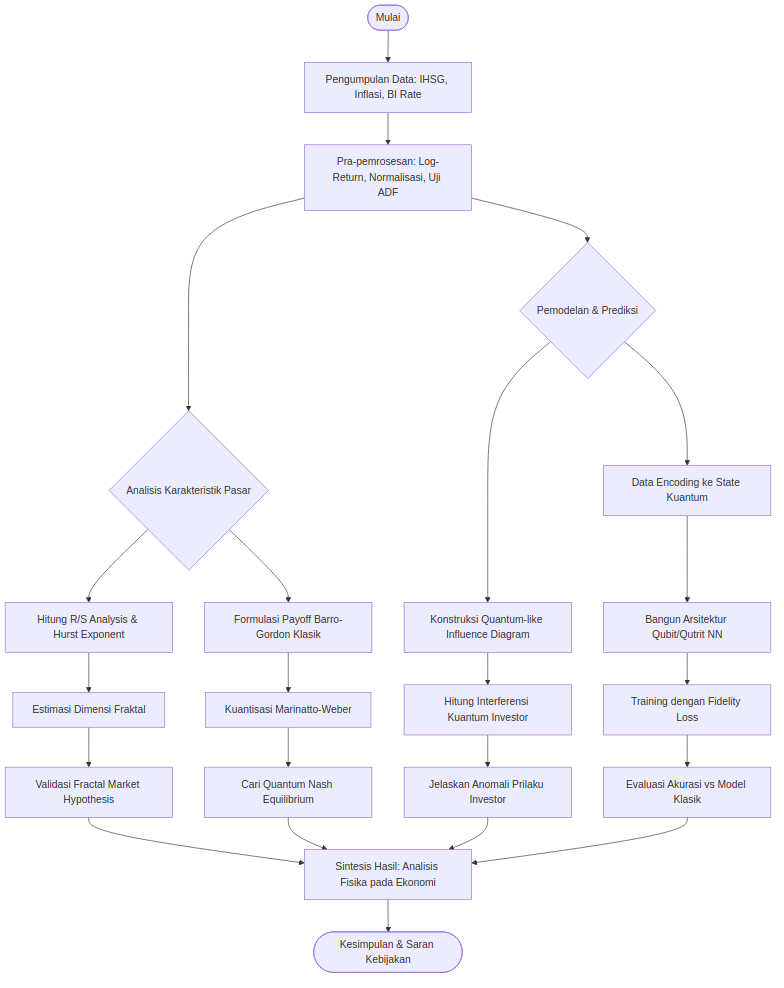
\includegraphics[width=0.9\textwidth]{Bab3/bab3_flowchart.png}
    \caption{Diagram Alir Penelitian}
    \label{fig:flowchart}
\end{figure}